\documentclass[colorinlistoftodos]{article}

% if you need to pass options to natbib, use, e.g.:
% \PassOptionsToPackage{numbers, compress}{natbib}
% before loading nips_2018

\usepackage[final]{nips_2018}

\usepackage[utf8]{inputenc} % allow utf-8 input
\usepackage[T1]{fontenc}    % use 8-bit T1 fonts
\usepackage{hyperref}       % hyperlinks
\usepackage{url}            % simple URL typesetting
\usepackage{booktabs}       % professional-quality tables
\usepackage{amsfonts}       % blackboard math symbols
\usepackage{nicefrac}       % compact symbols for 1/2, etc.
\usepackage{microtype}      % microtypography


%-----------------------------------------------------------------
\usepackage{pdfpages}
\usepackage{float}
\usepackage{tikz}
\usetikzlibrary{positioning}
\usetikzlibrary{calc}

\usepackage{amssymb,amsmath}
\usepackage{mathtools}

\usepackage{color}
\usepackage[font=small,labelfont=bf]{caption}
%----------------
\usepackage{algorithm,algorithmicx,algpseudocode}
\algnewcommand\algorithmicinput{\textbf{Input:}}
\algnewcommand\INPUT{\item[\algorithmicinput]}
\algnewcommand\algorithmicoutput{\textbf{Output:}}
\algnewcommand\OUTPUT{\item[\algorithmicoutput]}
\algnewcommand\algorithmicidea{\textbf{Idea:}}
\algnewcommand\IDEA{\item[\algorithmicidea]}
\algnewcommand\algorithmicinit{\textbf{Initialize:}}
\algnewcommand\INIT{\item[\algorithmicinit]}
%----------------

\usepackage{amsthm}

\providecommand{\tightlist}{%
  \setlength{\itemsep}{0pt}\setlength{\parskip}{0pt}}

\usepackage{fancyvrb}

% pandoc tmp.markdown -t latex -o tmp.tex

\theoremstyle{definition}
\newtheorem{definition}{Definition}[section]
\def\R{\mathbb{R}}

\usepackage{wrapfig}
\usepackage{lipsum}  % generates filler text

\usepackage{todonotes}
\newcommand{\rob}[1]{\todo[color=red!40]{Rob: #1}}
%-----------------------------------------------------------------
\title{Biologically Plausible Deep Learning: \\
		A Critical Review of Guergiev et al. (2017)}

\author{
  Robert T. Lange \thanks{This progress report was submitted as part of the final project of the "Models of Neural Systems" (Winter Term 2018/2019) computer practical course taught and organized by Prof. Richard Kempter (Bernstein Center for Computational Neuroscience, Berlin).} \ \thanks{Our implementation and further documentation can be found here: \url{https://github.com/RobertTLange/Bio-Plausible-DeepLearning}. Parts of the code were taken from \url{https://github.com/jordan-g/Segregated-Dendrite-Deep-Learning}.} \\
  Einstein Center for Neurosciences Berlin\\
  \url{robert.lange17@imperial.ac.uk} \\
  \url{www.rob-lange.com} \\
}

\begin{document}


\maketitle

%--------------------------------------------------------------------


%--------------------------------------------------------------------
\section{Introduction}

Backpropagation \citep{rumelhart1986} provides a computationally efficient solution to the synaptic credit assignment problem in Deep Learning (see e.g. \citet{lecun2015, schmidhuber2015}). Furthermore, deep neural networks outperform alternatives in modeling activity patterns in the visual cortex (see e.g. \citep{yamins_2016, khaligh_2014}).
While computational graphs and the chain rule successfully calculate gradients in deep layered structures, the mere empirical success does not imply that the brain is capable of implementing such a procedure. In order to understand why backpropagation might still provide an approximation to the neural credit assignment solution, we need to better understand the underlying mechanisms and alternatives.
In this report we review different approaches which intend to solve the credit assignment problem in a biological plausible fashion. We focus on an approach which implements a local plasticity rule in feedforward neural networks  with dendritic compartments \citep{guerguiev2017}.

\citet{larkum_1999}, first, highlighted the importance of electrical segregation of apical dendritic integration in pyramidal neurons in layer 5 of the neocortex. The calcium-rich apical shaft receives inputs from higher cortical areas which in turn can lead to prolonged activity in the form of plateau potentials. These potentials propagate down to the soma where they are assumed to drive plasticity. The basal compartment, on the other hand, receives bottom-up input from lower-level sensory areas. \citet{kording2001}, therefore, proposed that a learning rule based on the integration of both such signals might solve the credit assignment problem. \citet{guerguiev2017} took this initial inspiration to the workbench, introduced a feedforward-specific formulation and successfully tested its implementation on a basic MNIST benchmark.   
It has been argued that such a learning rule overcomes multiple points of critique while accomplishing similar strong results. But does it scale to more complex datasets? How robust is this new credit assignment paradigm? Ideally, the learning rule does not require vast amounts of hyperparameter tuning. Hence, we conduct robustness checks and analyze the learning dynamics across three different datasets.

The report is structured as follows: First, we introduce notation as well as fundamental problems with backpropagation. We briefly review the literature trying to solve such concerns.
Afterwards, we outline the local compartmental learning paradigm introduced in \citet{guerguiev2017}. We show how a simplified model of plateau potentials generated at the apical shaft can be used to obtain local objective functions.
Furthermore, we empirically analyze the proposed framework and conduct experiments with different complexities of datasets. Furthermore, we analyze the convergence behavior and hyperparameter robustness of the learning rule as compared to standard backpropagation.
Finally, we discuss problems with the proposed approach and discuss recent contributions to the literature as well as ideas to solve such problems.



%--------------------------------------------------------------------
\newpage
\section{Credit Assignment in Deep Layered Structures}

Arguably, Deep Learning's most simple, layered architecture is the Multi-Layer Perceptron (MLP). A MLP composes layers $l=1, \dots, L$ of non-linear and affine transformations:\footnote{For clarity and completeness we follow \citet{bartunov2018}'s notation throughout this manuscript.}

$$h_l \coloneqq f(h_{l-1}; \theta_l) = \sigma_l (W_l h_{l-1} + b_l)$$ 

where $h_0 = x$ and $\theta_l = \{W_l, b_l\}$. In a classification task the final output layer $h_L$ represents the output distribution over the possible labels. In order to train such a composition one has to define a loss function. A standard supervised classification loss function might be given by the cross-entropy between the actual labels distribution, $q(y|x)$, and the output distribution of the network, $p(y|h_L)$:

$$\mathcal{L}(h_L) = - \sum_y q(y|x) log p(y|h_L)$$

In order to train the parameters $\Theta \coloneqq \{\theta\}_{l=1}^L$ of a network, one makes use of powerful auto-differentiation tools and stochastic/batch gradient descent methods. More specifically, the classical backpropagation algorithm is based on the following derivation:

\begin{align*}
	\frac{\partial \mathcal{L}}{\partial \theta_l} &= \left(\frac{dh_{l}}{d \theta_{l}}\right)^T \frac{\partial \mathcal{L}}{\partial h_{l}} = \left(\frac{dh_{l}}{d \theta_{l}}\right)^T \left(\frac{dh_{l+1}}{d h_{l}}\right)^T \frac{\partial \mathcal{L}}{\partial h_{l+1}} \\ 
	&=  \left(\frac{dh_{l}}{d \theta_{l}}\right)^T \underbrace{\left(W_{l+1} diag\left(\sigma_{l+1}'(W_{l+1}h_l +b_{l+1})\right)\right)^T}_{\coloneqq \delta_{l+1}} \frac{\partial \mathcal{L}}{\partial h_{l+1}} \\
	&= \left(\frac{dh_{l}}{d \theta_{l}}\right)^T \delta_{l+1} \delta_{l+2}\frac{\partial \mathcal{L}}{\partial h_{l+2}} = \dots =  \left(\frac{dh_{l}}{d \theta_{l}}\right)^T \left(\prod_{i=l+1}^L \delta_i\right) \frac{\partial \mathcal{L}}{\partial h_{L}}
\end{align*}

In order to compute the gradient with respect to the parameters of a specific layer $l$, one first computes a forward pass through the network to obtain the hidden units $\{h_l\}_{l=0}^L$. Afterwards, one computes a loss-based error signal, $e \coloneqq \frac{\partial \mathcal{L}}{\partial h_{L}}$ based on the true label. Ultimately, the weights are updated using a standard stochastic gradient descent rule with learning rate $\eta$:

$$\Delta \theta_l \coloneqq \eta \times \frac{\partial L}{\partial \theta_l}$$

While computationally efficient, there are multiple problems rendering backpropagation biologically implausible: 

\begin{enumerate}
	\item Weight transport problem: Downstream errors are fed back to the upstream neurons via an exact symmetric copy of the downstream synaptic weight matrix. This amounts to each neuron "deep" within the network having access to precise knowledge of all downstream synapses.
	\item Global signed error signals: The error computed via forward propagation $e$ has to be accessible at every layer. Physiologically, it is not clear how this can be achieved without a separate pathway.
	\item Costly matrix transposition: Depending on the memory constraints, matrix transposition is a costly permutation operation. This might be circumvented by accessing the synaptic weights in a different order. Both options do not seem particularly plausible.
	\item Feedback information propagation does not influence the activity of the feedforward network. This does not align with any neuropyhsiological observation.
\end{enumerate}

Based on these observations, the neuroscience community has mostly dismissed the hypothesis of the brain being involved in something akin to deep learning. Still, there remain some efforts to overcome such weaknesses. In the following section we will review such approaches.

%--------------------------------------------------------------------
\newpage
\section{Literature Review}

Backpropagation assumes a very constraint feedback pathway and thereby introduces the weight transport problem. Feedback alignment \citep{lillicrap2016} overcomes this problem by completely loosening the constraints on the feedback channel. More specifically, the feedback synapses are set to be a fixed random matrix, $B$. Very astonishingly, \citet{lillicrap2016} were able to analytically and empirically show that credit is still assigned with such a learning rule.
Ultimately, the feedforward weights "align" such that the random matrix is capable to propagate valuable error-reducing information. More specifically, they exploit the fact that as long as $B \approx W^T$ and $e^TWBe > 0$, the gradient will be within 90 degrees of the optimal backpropagation gradient. Hence, the rough direction will be correct and only the speed of learning depends on the exact degree of divergence.
The learning rule is able to approximate simple linear functions, can be extended with sigmoid non-linearities to tackle classification problems and can also accommodate for sparsity. Still, feedback alignment does require the propagation of a signed error signal via a distinct pathway. This does not seem completely plausible and provides the motivation for \citet{guerguiev2017} multi-compartment approach. Finally, artificial neurons in the feedback alignment setup do not integrate activity over time nor spike stochastically.
While feedback alignment relies on an implicit feedback communication, target propagation \citep{lecun_1986} trains a separate set of parameters $\{\lambda_l\}_{l=1}^L$ which explicitly defines backward activity $g(.; \lambda_l)$.
The weights are learned by minimizing a reconstruction loss akin to how autoencoders are trained. Hence, the feedback (decoding) connections are tuned to invert the preceding feedforward (encoding) activity. Thereby, the forward and backward weights are learned simultaneously, which can lead to destabilized learning.
Versions of target propagation differ in the construction of the decoding target. E.g. difference target propagation \citep{lee2015} makes use of a simple stabilized delta rule to construct the inverse operation.  

$$\hat{h}_l = g(\hat{h}_{l+1}; \lambda_{l+1}) + \left(h_l - g(h_{l+1}; \lambda_{l+1})\right)$$

Note that this does not hold for the final layer, where the gradient is explicitly computed. This ensures enough variability in the gradients even if the data distribution has low entropy.
Simplified difference target propagation \citep{bartunov2018}, on the other hand, overcomes this biologically implausible gradient by setting $\hat{h}_L = arg\min \mathcal{L}(h_L)$. \citet{bartunov2018} highlights that low entropy in the classification targets can potentially lead to non-robust inverse weights.
Figure \ref{fig:lit_rev} provides a more detailed summary of the existing literature:

\begin{figure}[H]
	\centering
	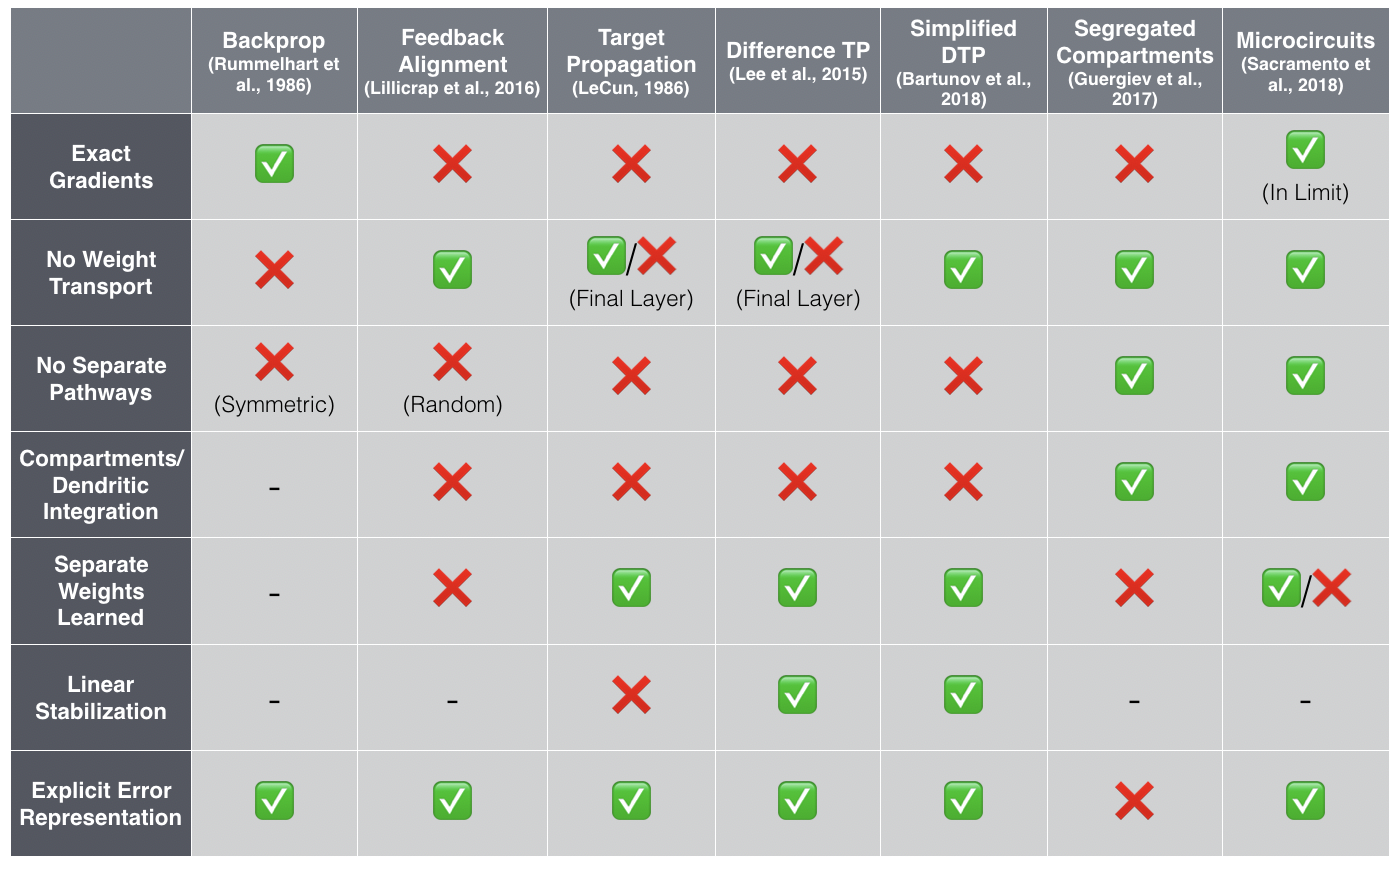
\includegraphics[width=\textwidth]{../figures/report/lit_rev}
	\caption{Literature Review.}	\label{fig:lit_rev}
\end{figure}

%--------------------------------------------------------------------
\newpage
\section{Local Synaptic Learning Rules with Dendritic Integration}

\citet{kording2001} postulated that the brain might solve the credit assignment problem with the help of electrical segregation. Inspired by the physiological traits of multi-compartmental pyramidal neurons (see figure \ref{fig:pyramidal}), they derive a basic local learning rule which integrates top-down feedback at the distal apical dendrites with bottom-up sensory input from the basal dendrites. 
\citet{guerguiev2017} extend this intuition to the assignment of credit in MLPs. More specifically, they formalize the idea of plateau potentials driving synaptic plasticity in pyramidal neurons. The apical compartment does not constantly communicate with the somatic compartment. Instead, voltage-gated $Ca^{2+}$ channels provide feedback information to the nucleus. Plateau potentials, thereby, correspond to a long-lasting increase in membrane potential due to such events in the apical shaft. 

\begin{figure}[H]
\centering
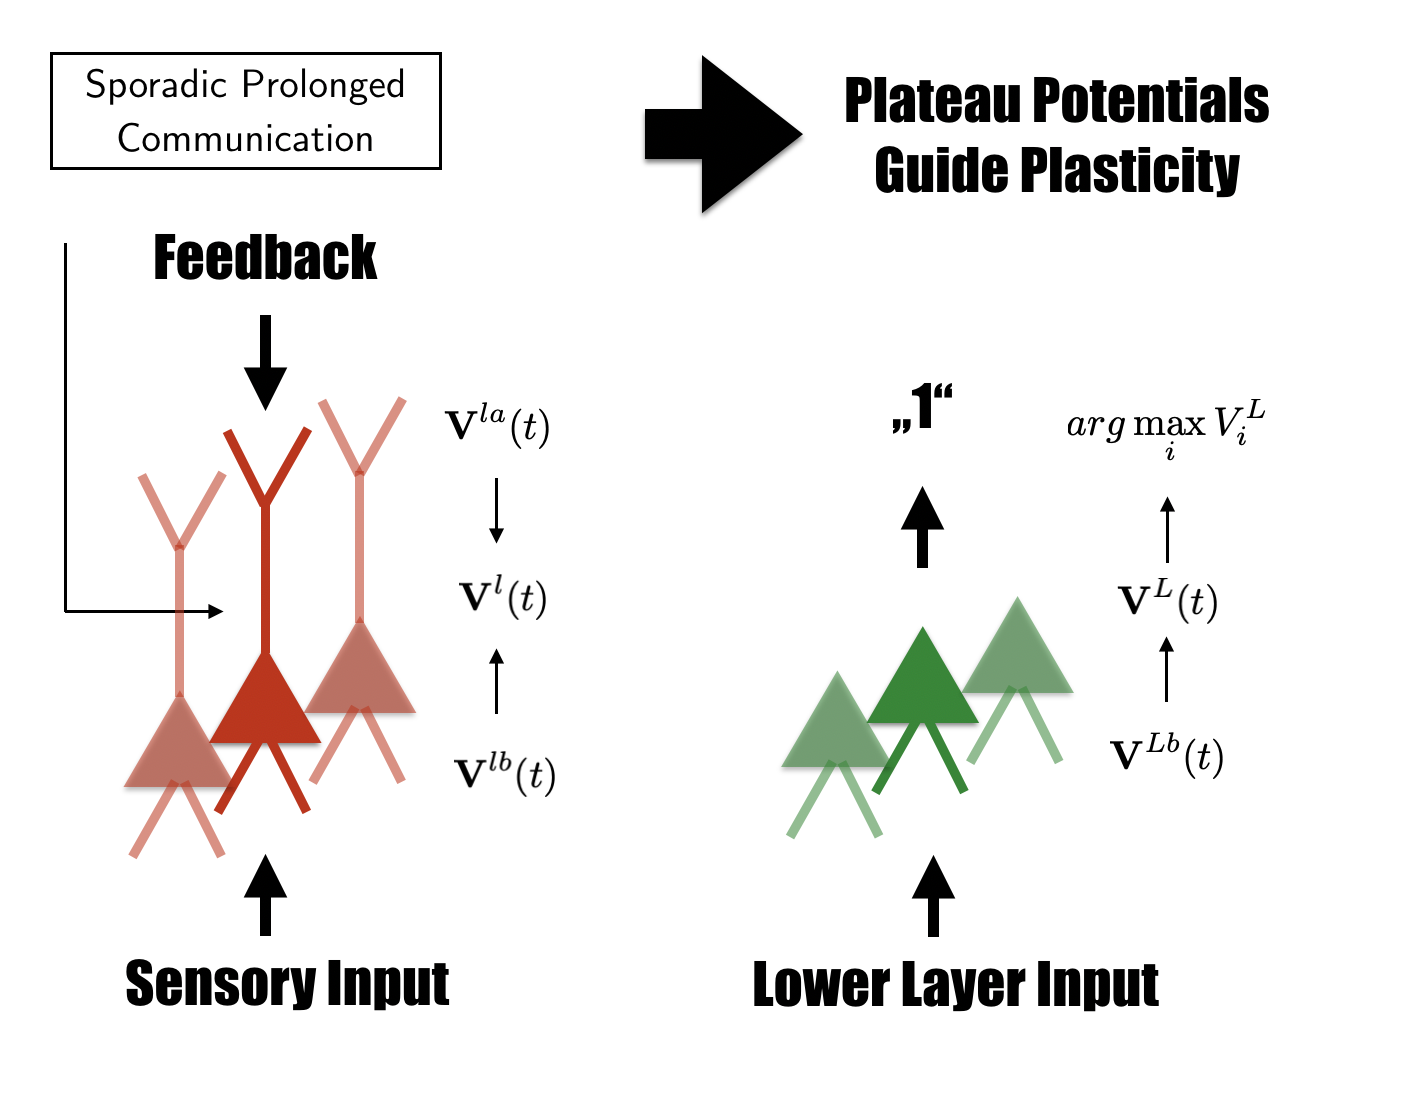
\includegraphics[width=0.75\textwidth]{../figures/report/elec_seg_3}
\caption{\label{fig:pyramidal} A schematic illustration of compartmental hidden and output layer neurons.}
\end{figure}
 
Let $n_{l}$ denote the number of hidden units in layer $l$. A hidden layer is described by real-valued vectors $\mathbf{V^{la}}(t), \mathbf{V^{lb}}(t), \mathbf{V^{l}}(t) \in \mathbb{R}^{n_l}$ which correspond to the three compartments of each neuron:

\begin{align*}
	\textit{Apical:  } \mathbf{V^{la}}(t) &= [V_1^{la}(t), \dots, V_{n_l}^{la}(t)]\\
	\textit{Basal:  } \mathbf{V^{lb}}(t) &= [V_1^{lb}(t), \dots, V_{n_l}^{lb}(t)]\\
	\textit{Somatic:  }\mathbf{V^{l}}(t) &= [V_1^{l}(t), \dots, V_{n_l}^{l}(t)]
\end{align*}

Assuming that the resting membrane potential is at 0 ($V^l_{rest}=0$), the somatic membrane potential of the hidden layer evolves based on top-down apical dendritic and bottom-up basal dendritic inputs. 
These basal input is computed via a dot-product between the forward weights $W^l$ and the the kernel-filtered spike train $s^{l-1}$ from the previous layer and by adding an intercept $b^l$. The initial spike train, $s^0 = s^{input}$, is given by a Poisson process whose rate-of-fire is determined by the pixel intensity of a given input image. 
The apical input, on the other hand, is computed by a dot-product between the feedback weights $Y$ and the upper layer spike train $s^{l+1}$. Both contributions are scaled by the ratio of dendritic conductances $g_a, g_b$ and the leak conductance $g_{leak}$. Please note that these quantities do not exhibit any biologically meaningful units of measurement and can hardly be set by physiological intuition/evidence.
The dynamics are then summarized by the following system of equations:

	\begin{align*}
		\tau \frac{dV_i^l(t)}{dt} = -V_i^l(t) + \frac{g_b}{g_{leak}}\left(V_i^{lb}(t) - V_i^l(t)\right) +\frac{g_a}{g_{leak}}\left(V_i^{la}(t) - V_i^l(t)\right)\\
		V_i^{lb} = \sum_{j=1}^{n_{l-1}} W_{ij}^l s_j^{l-1}(t) + b_i^l; \ \ \ V_i^{la} = \sum_{j=1}^{n_{l+1}} Y_{ij}^l s^{l+1}_j(t); \ \ \
		s_j^{l}(t) = \sum_k \kappa(t-t_{jk}^{l})
	\end{align*}

where $\kappa$ denotes a response kernel that convolves the spike train (e.g. exponential).
	
The output layer indexed by $L$, on the other hand, does not receive any apical inputs and thus consists of only two compartments: $\mathbf{V}^{Lb}(t), \mathbf{V}^{L}(t) \in \R^n$ with dendritic conductance $g_d$. 

\begin{align*}
		\tau \frac{dV_i^L(t)}{dt} &= -V_i^L(t) + \frac{g_d}{g_{leak}}\left(V_i^{Lb}(t) - V_i^L(t) \right) + I_i(t)\\
		V_i^{Lb} &= \sum_{j=1}^{n_{L-1}} W_{ij}^L s_j^{L-1}(t) + b_i^L
\end{align*}

Classifications are obtained by integrating until settlement and selecting the label corresponding to the output neuron with the largest rate-of-fire (where $\phi_{max}$ denotes max-firing):

$$arg\max_i \phi^L_i(t) = \phi_{max} \sigma(V_i^L(t))$$

The somatic output current also receives an external teaching current, $I_i(t)$, which guides learning. More specifically, learning is defined by two phases of varying length: A forward and a target phase (see figure \ref{fig:phases}). The length of such phases are randomly sampled from an inverse Gaussian distribution.\footnote{\citet{guerguiev2017} argue that the specific length does not matter. Important is only the existence of these those alternating phases.}
More specifically, let the forward phase start at time $t_0$. There is assumed to be an initial settling period of $\Delta t_s$.

\begin{figure}[H]
\centering
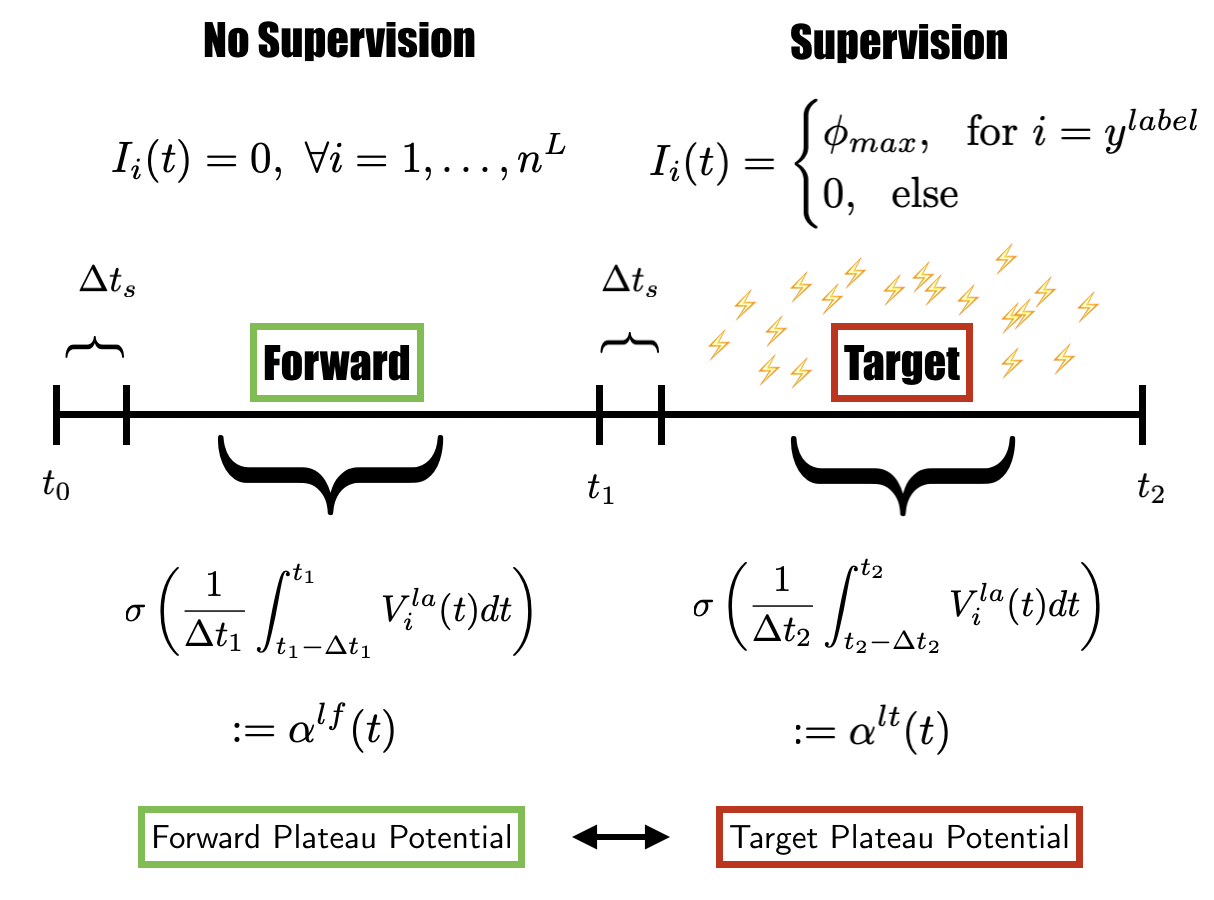
\includegraphics[width=0.75\textwidth]{../figures/report/phases_3}
\caption{\label{fig:phases} Two Phase Learning with Segregated Compartments}
\end{figure}	
 
During the forward phase the teaching current is set to zero for all output neurons, i.e. $I_i(t) = 0, \ \forall i=1,\dots, n^L$. For the time from $t_0 + \Delta t_s$ until the start of the target phase $t_1$ we calculate an approximation of the plateau potential by averaging over the apical membrane potential and taking the sigmoid non-linearity, $\sigma(.)$, of the resulting value.
During the target phase from $t_1 + \Delta t_s$ until $t_2$ we do the same, expect for the fact that the external current is set to a maximal firing rate $\phi_{max}$ for the specific label of the currently processed image, $I_i = \phi_{max}$ for $i = y_{label}$ and 0 otherwise. Thereby, the teaching current nudges the activity of the network towards the correct output.
	
\begin{align*}
	\text{Forward:  } \alpha_i^{lf} &= \sigma\left(\frac{1}{\Delta t_1} \int_{t_1 - \Delta t_1}^{t_1} V_i^{la}(t)dt\right) \text{  with  } I_i(t) = 0, \ \forall i=1,\dots, n^L, l=0,\dots, L-1 \\
	\text{Target:  } \alpha_i^{lt} &= \sigma\left(\frac{1}{\Delta t_2} \int_{t_2 - \Delta t_2}^{t_2} V_i^{la}(t)dt\right) \text{  with  } I_i(t) = \phi_{max}, \ \text{for  } i = y_{label}, 0 \text{  otherwise.}
\end{align*}

So how can learning be defined in such a model? \citet{guerguiev2017} argue that a network which has learned to classify, exhibits the same activity pattern during the forward phase (i.e. without teaching current/supervision signal) as in the supervised target phase. More formally, the somatic compartments generating Poisson-like spikes should fire at the target rate, $\phi_i^{L\star} = \frac{1}{\Delta t_2} \int_{t_1 + \Delta t_s}^{t_2} \phi_i^L(t)dt$. A desired loss function for the output layer can then be derived as follows:

$$\mathcal{L}^L = ||\phi^{L\star} - \bar{\phi}^{Lf}||_2^2 = ||\frac{1}{\Delta t_2} \int_{t_1 + \Delta t_s}^{t_2} \phi^L(t)dt - \frac{1}{\Delta t_1} \int_{t_0 + \Delta t_s}^{t_1} \phi^L(t)dt||_2^2$$

For all other layers the loss function is defined in terms of the approximate plateau potential difference:

$$L^l = ||\phi^{l\star} - \bar{\phi}^{lf}||_2^2 = ||\bar{\phi}^{lf} + \alpha^{lt} - \alpha^{lf} - \bar{\phi}^{lf}||_2^2 = ||\alpha^{lt} - \alpha^{lf}||_2^2 \ \forall l=0, \dots, L-1$$

Given such layer-wise loss functions, one can then perform local gradient descent updates in order to tune the feedforward synaptic weights:

$$\Delta W^l \propto \frac{\partial \mathcal{L}^l}{\partial W^l} \text{  and  } \Delta b^l \propto \frac{\partial \mathcal{L}^l}{\partial b^l}$$

Please note that one can also learn the feedback weights $Y^l$, obtaining a compartmental version of target propagation. When keeping $Y^l$ fixed to their random initialization one, on the other hand, obtains a learning rule akin to feedback alignment.

%--------------------------------------------------------------------
%\newpage
\section{Empirical Investigations}

\begin{figure}[H]
	\centering
	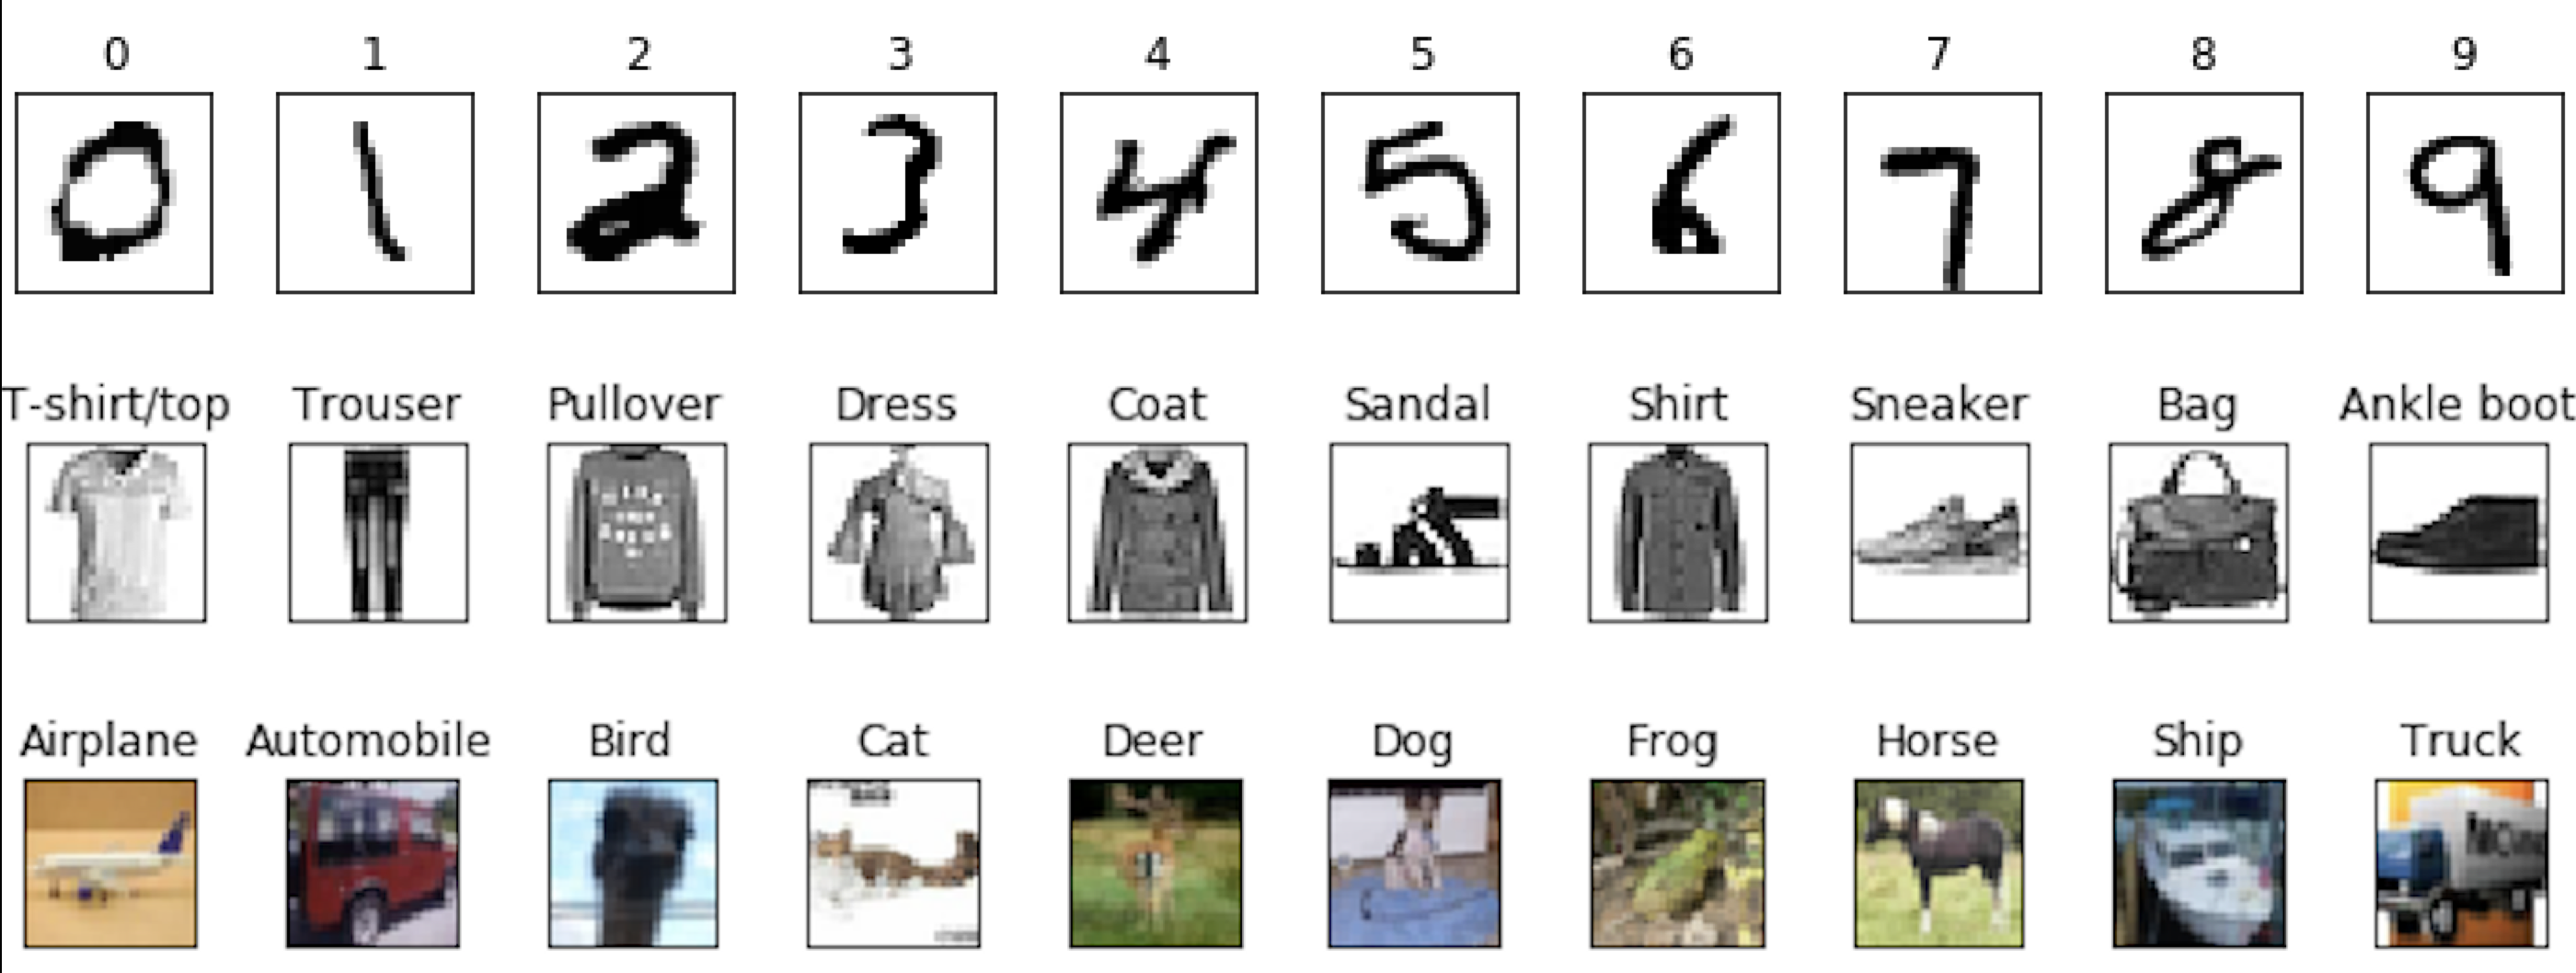
\includegraphics[width=\textwidth]{../figures/report/datasets}
	\caption{Illustration of the 10 different classes/labels of the analyzed datasets. \textbf{Top Row:} MNIST dataset. \textbf{Middle Row:} Fashion-MNIST dataset. Data format: $70000 \times 1 \times 28 \times 28$. \textbf{Bottom Row:} CIFAR-10 dataset. Data format: $60000 \times 3 \times 32 \times 32$. From top to bottom the intra-class variability/entropy increases significantly. We normalize the pixel values to lie within $[0, 1]$ and reshape the images into vector format (e.g. $X \in [0, 1]^{784}$) before training the classifiers.}	\label{fig:data}
\end{figure}

Most of the computational neuroscience literature working on supervised learning focuses on a single dataset: MNIST \cite{lecun_1998}. Since object recognition tasks do not only require the skill of optical character recognition, we test the scalability and flexibility of the introduced architecture to different datasets. It is desirable to have a learning rule which is able to deal with dataset which exhibit large amounts of entropy in their data generating process. Therefore, we implemented and tested the \citet{guerguiev2017} model not only on MNIST but also on the Fashion-MNIST \citep{xiao_2017} as well as the CIFAR-10 \citep{torralba_2008} dataset (see figure \ref{fig:data}). Figure \ref{fig:performance} compares the learning performance of the compartmental deep neural network with a standard backpropagation MLP and convolutional neural network (CNN). One can clearly observe that the alternative compartment-based learning rule accomplishes strong performance on both traditional MNIST and Fashion-MNIST. For the RGB CIFAR-10 dataset the compartmental approach falls drastically short. The validation accuracy does not exceed 35 percent after 10 epochs (SGD loops over the entire training dataset) compared to 45 percent for the backpropagation-based MLP.
Hence, this provides evidence that the approach proposed does not deal well with datasets which exhibit large variability in their representations.

\begin{figure}[H]
	\centering
	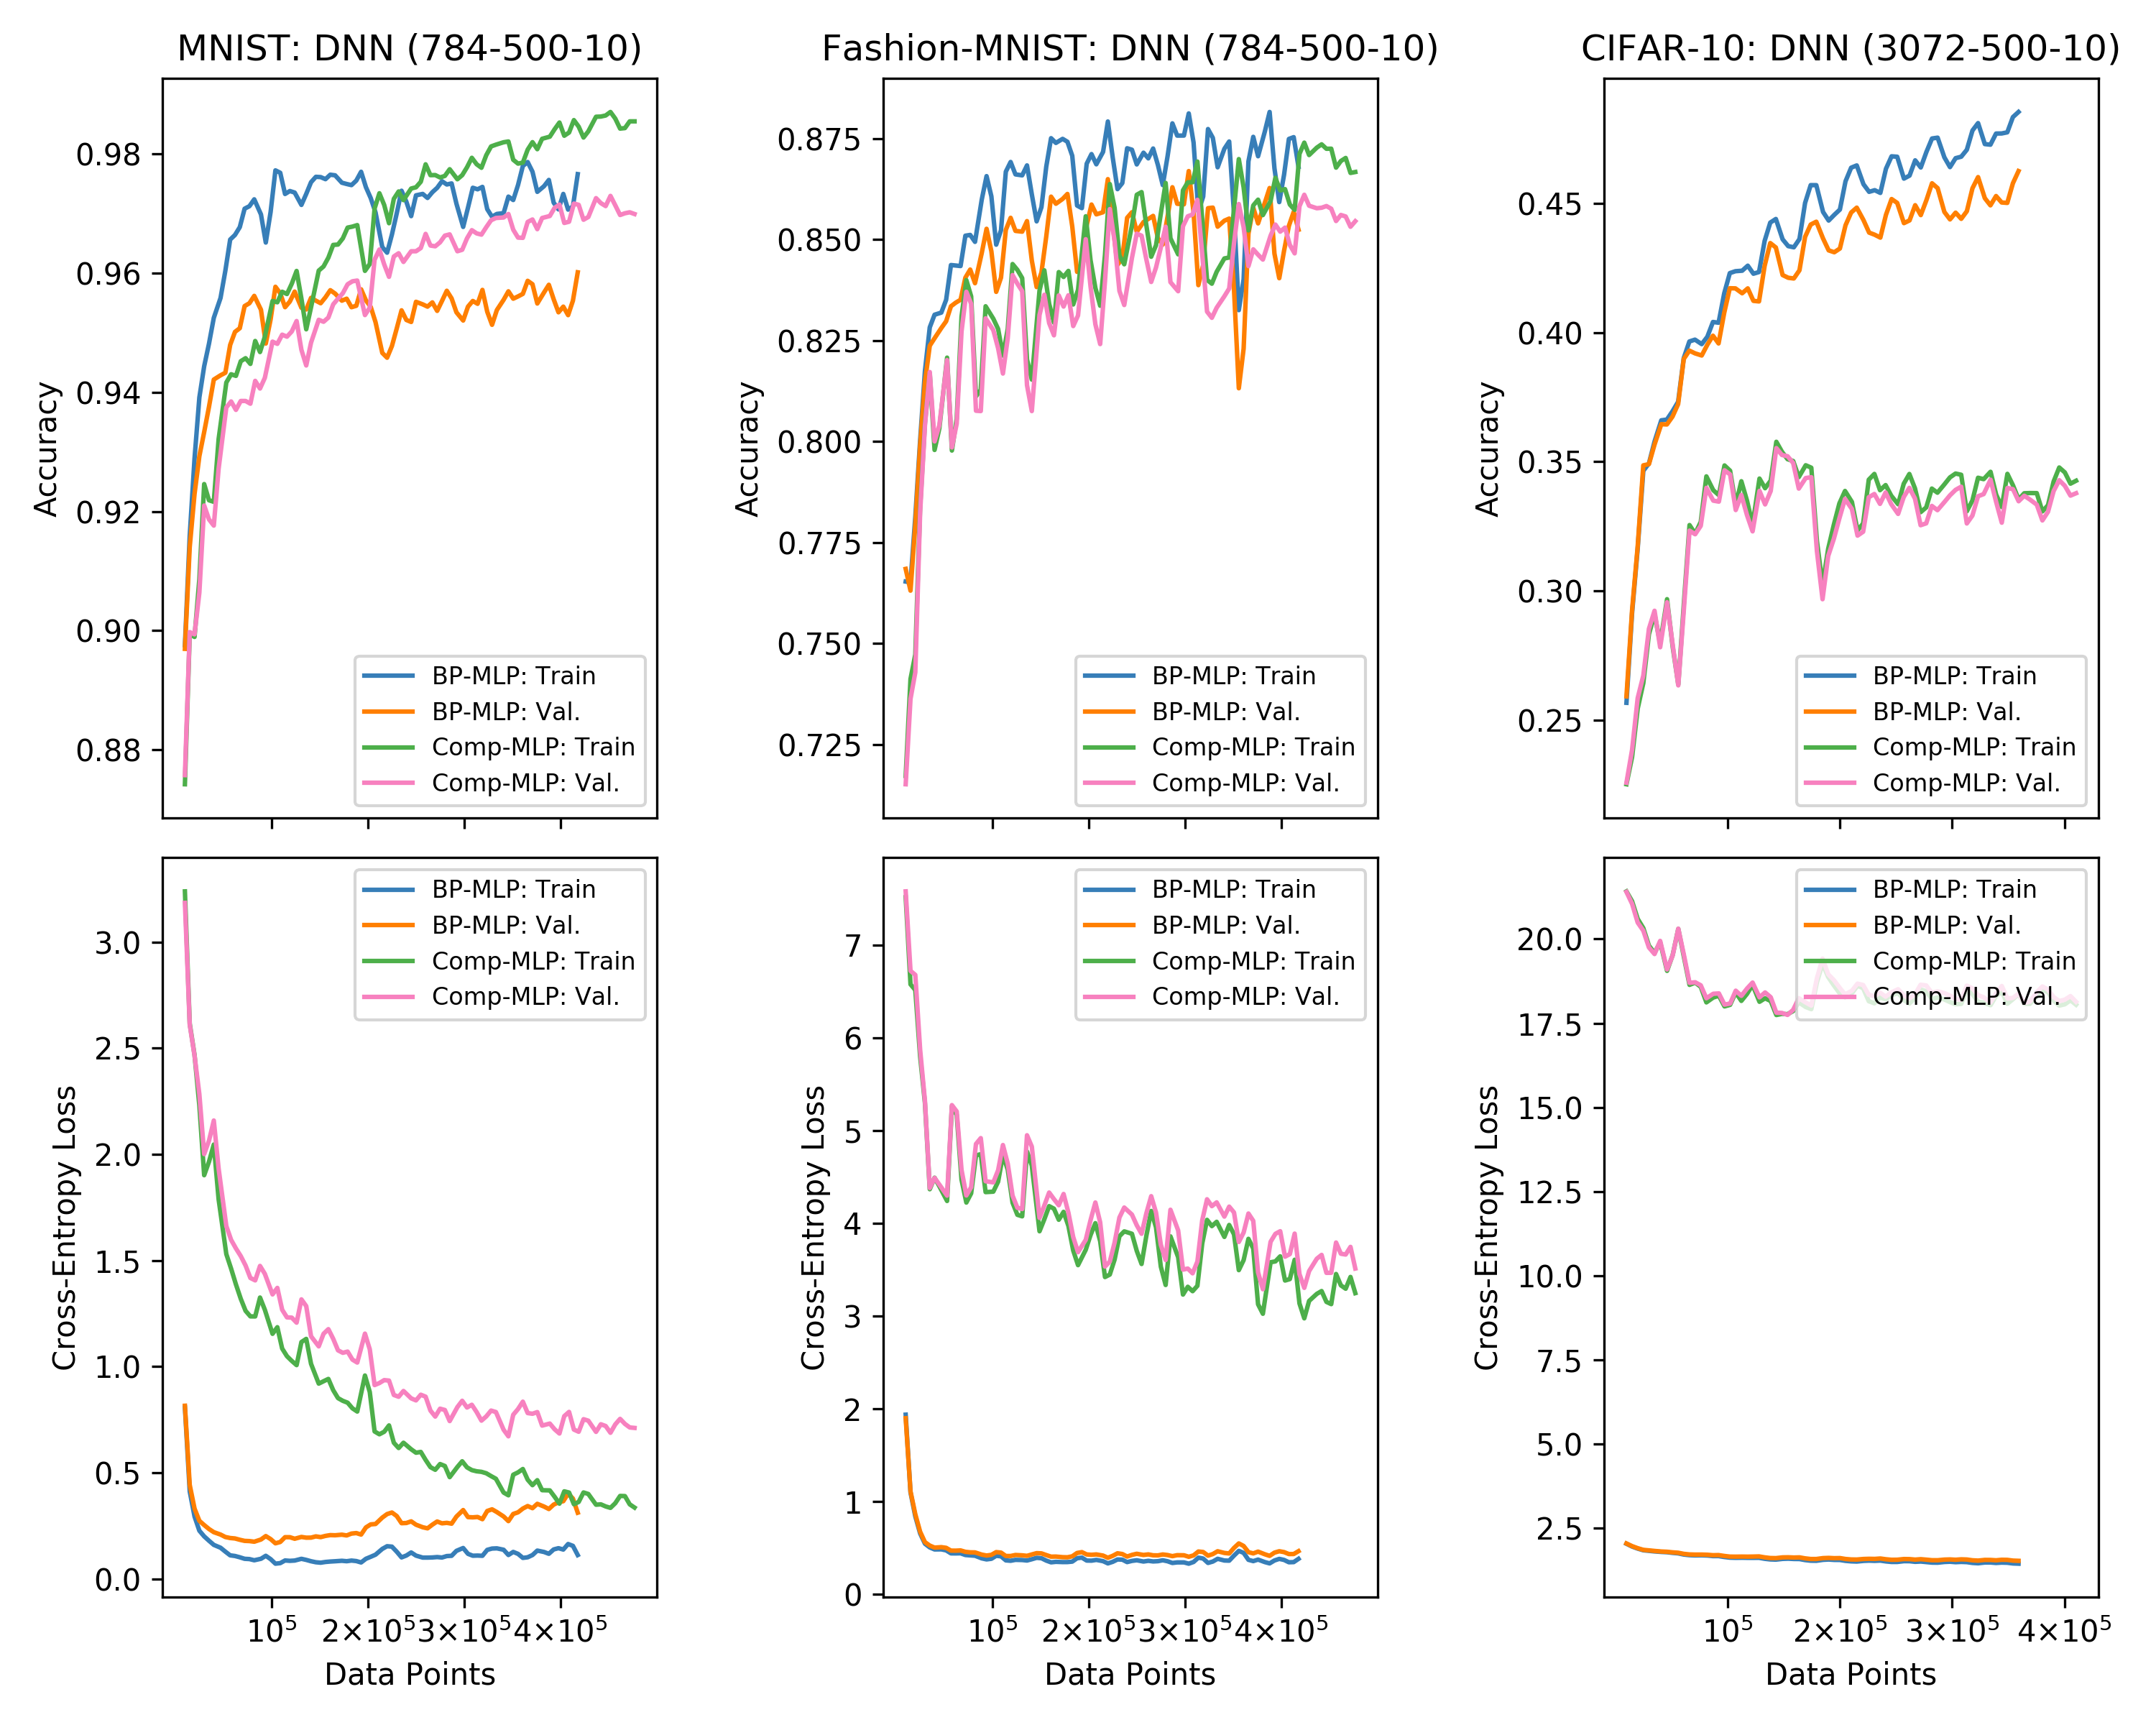
\includegraphics[width=\textwidth]{../figures/learning}
	\caption{Illustration of the learning performance. \textbf{Top Row}: Train and validation accuracy across the three datasets. \textbf{Bottom Row}: Train and validation cross-entropy loss across the three datasets. The MLP architectures consists of a single hidden layer with 100 hidden units.} \label{fig:performance}
\end{figure}


\subsection*{Learning Dynamics}

We further analyze the dynamics of the parameters across the learning process. The first row of figure \ref{fig:dynamics} displays the Frobenius norm of the weight matrix of the first layer. Large weights usually provide an indicator of overfitting (and thereby provide the motivation for norm-based regularization). One can observe that the weights are magnitudes larger for the compartmental DNN as compared to the backpropagation MLP. At the same time the weights appear to converge faster. The second row displays the relative change of the weights between updates. Finally, the gradients do not appear to change as much for the compartmental rule.
Together with out previous conclusions from the learning performance provides evidence for a local optimum being reached fairly early in the learning procedure. This might be the reason for strong performance early in the learning but is not desired later on.

\begin{figure}[H]
	\centering
	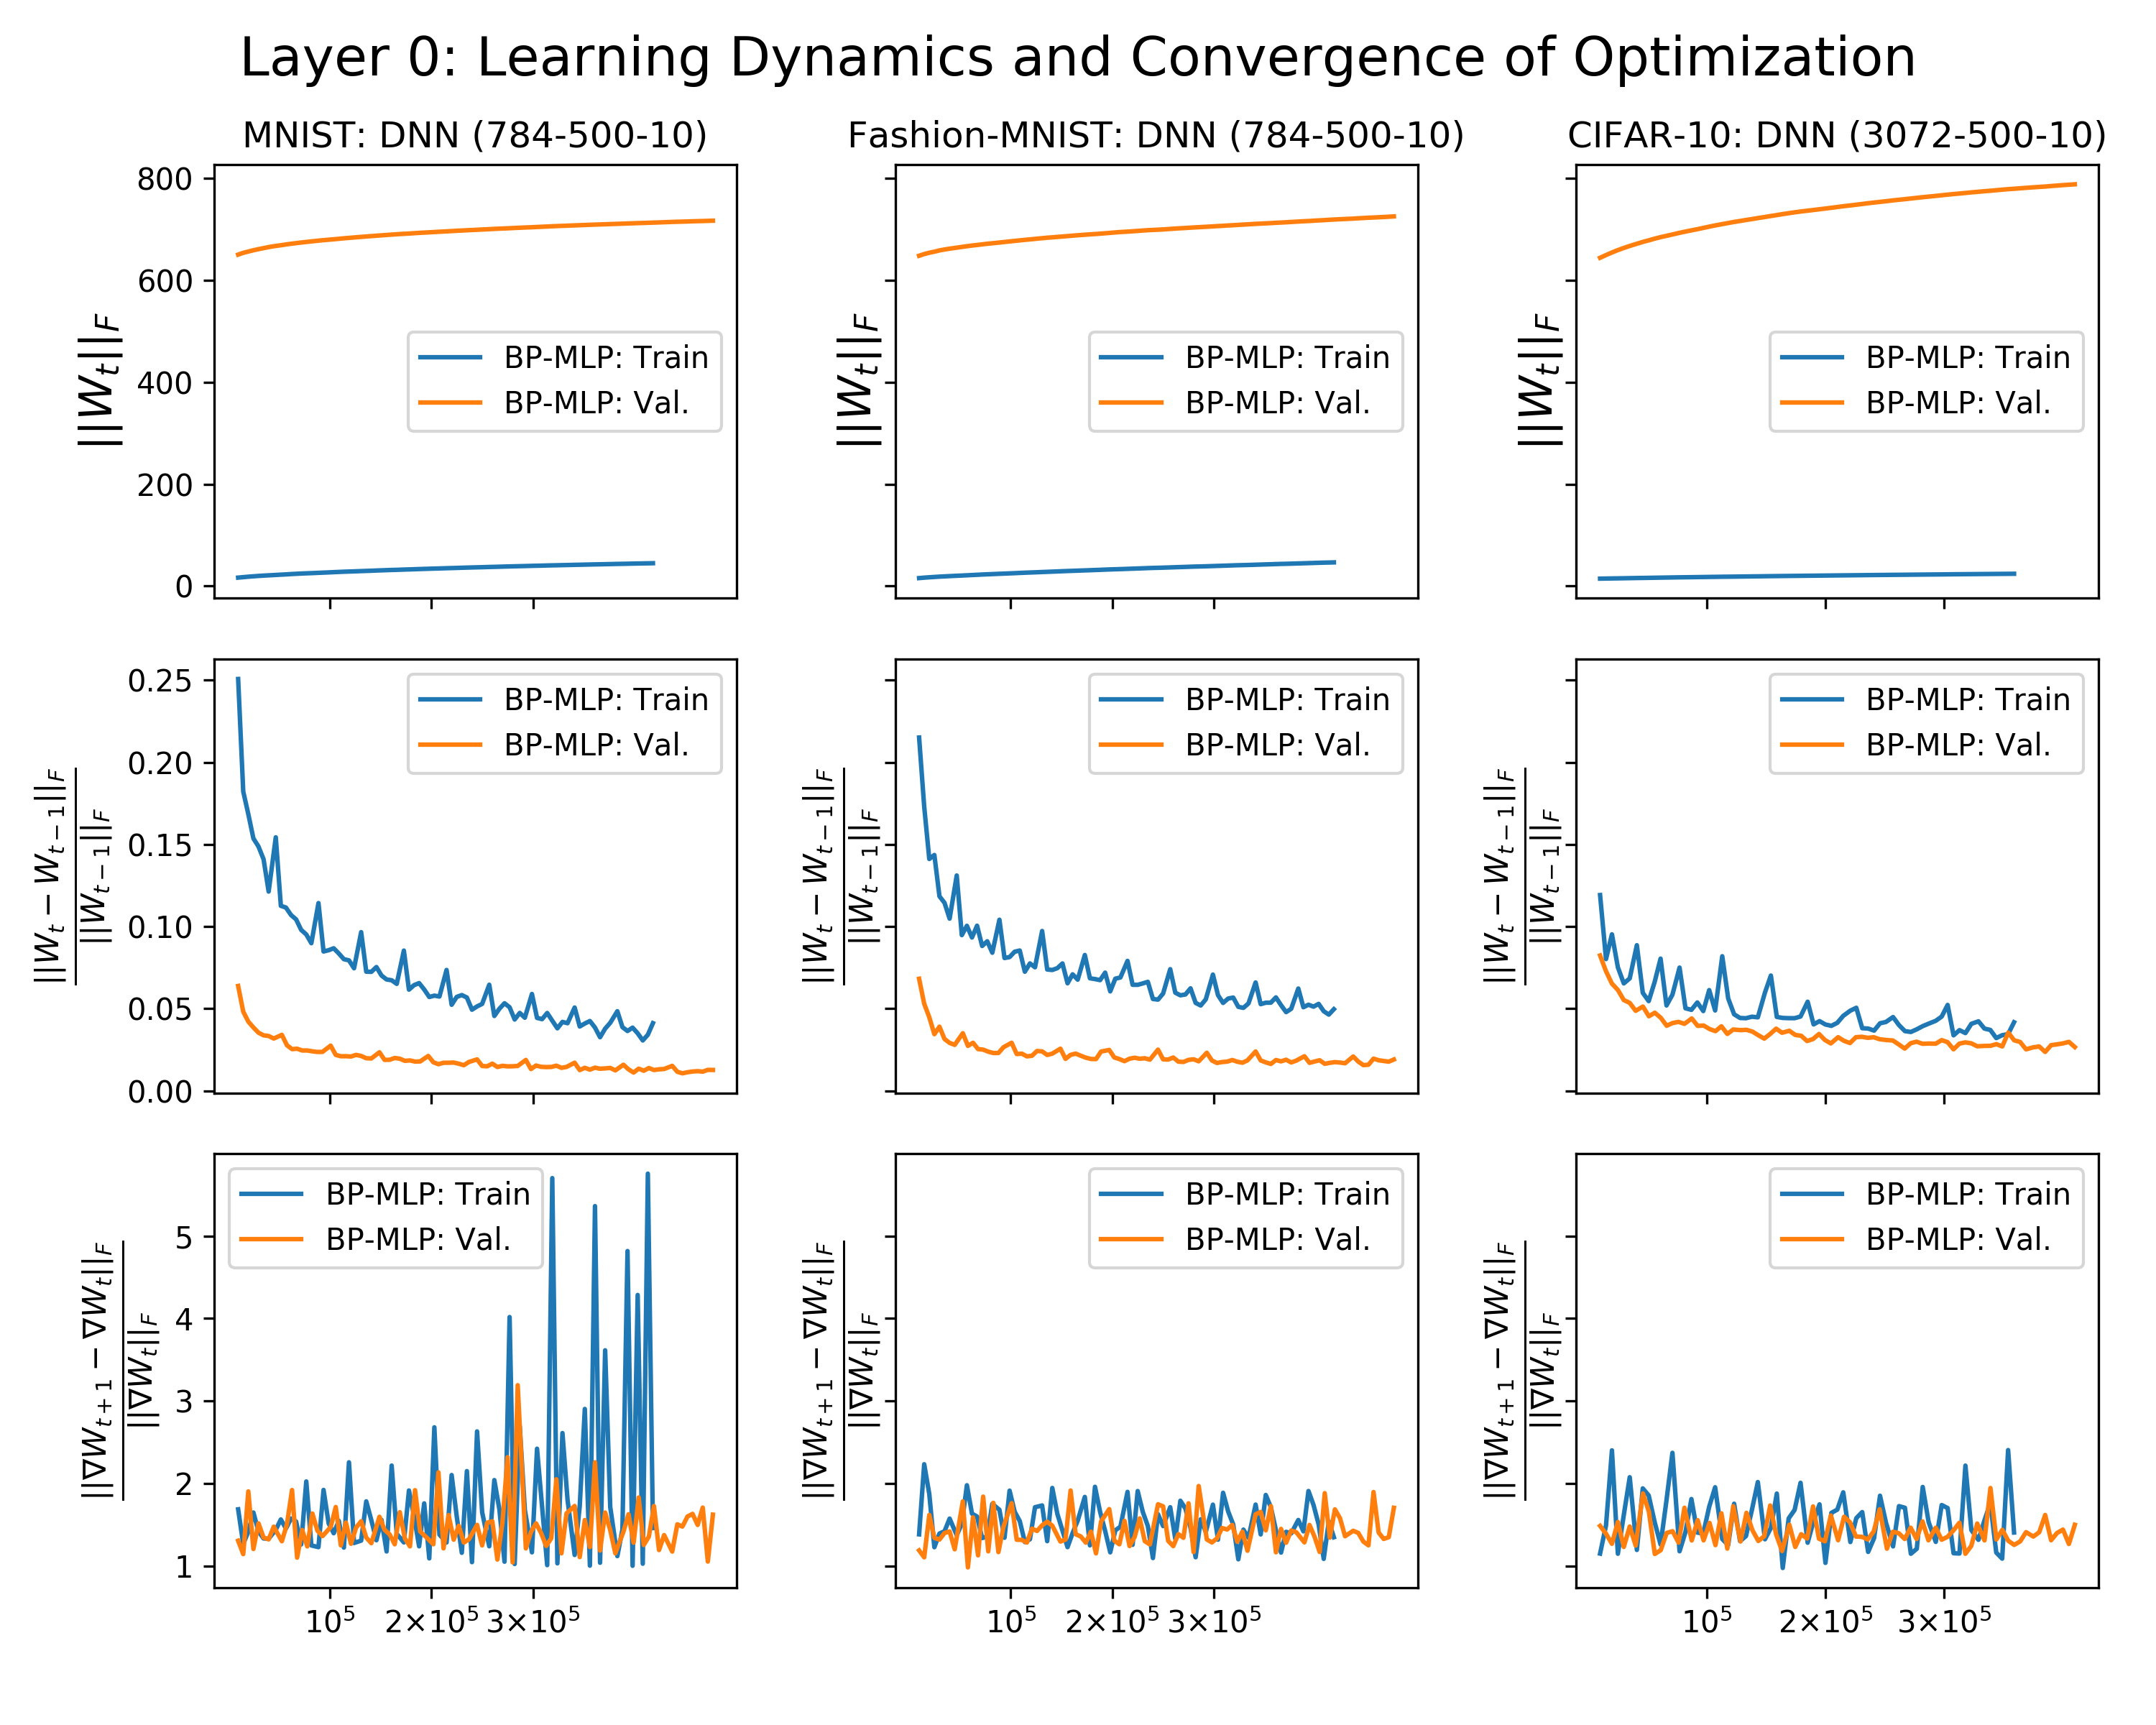
\includegraphics[width=\textwidth]{../figures/dynamics_l0}
	\caption{Illustration of the learning dynamics.}\label{fig:dynamics}
\end{figure}


\subsection*{Hyperparameter Robustness}

Finally, we are interested in the robustness of the compartmental approach. There are many hyperparameters which do not come with a natural biological interpretation (do to the rescaling of the membrane potential at rest). In the supplementary material we provide a list of all hyperparameters which have to optimized for a given classification task. An algorithmic approach to the credit assignment problem has to be robust to changes in such parameters. We therefore analyze the hyperparameter sensitivity with the help of Bayesian optimization.
Bayesian optimization (BO; \citet{snoek_2012}) is a probabilistic technique commonly used to optimize the parameters of complex functions with costly evaluations. Computing cross-validated test accuracies of deep networks is one such costly function. Instead of randomly searching through the hyperparameter space, one is able to guide the search in a Bayesian fashion. We approximate the loss function $\mathcal{L}^{k-fold}(\theta|X, y)$ as an infinitely dimensional vector with the help of a Gaussian Process (GP; see e.g. \citet{rasmussen_2004}). The properties (i.e. smoothness, differentiability, etc.) of the function are encoded in the covariance matrix of the GP. This in turn is characterized by a kernel function (e.g. squared-exponential or Matern). Given a mean vector and a covariance matrix, we can construct the multivariate Gaussian posterior of the loss surface given the data and as a function of the hyperparameters. 
The next hyperparameter configuration which we intend to evaluate has to efficiently tradeoff the mean (exploitation) and the variance (exploration) of the GP. This is usually done by evaluating an acquisition function (e.g. expected improvement, upper-confidence bound). Hence, instead of randomly evaluating the target function, we query the function in a Bayesian optimal fashion.\footnote{Note that the covariance matrix inversion needed to obtain the GP posterior comes at $\mathcal{O}(n^3)$ where $n$ denotes the number previous evaluations.} This query schedule reduces the number of overall network training but requires us to update the GP posterior after every evaluation and to evaluate the acquisition function.

\begin{figure}[H]
	\centering
	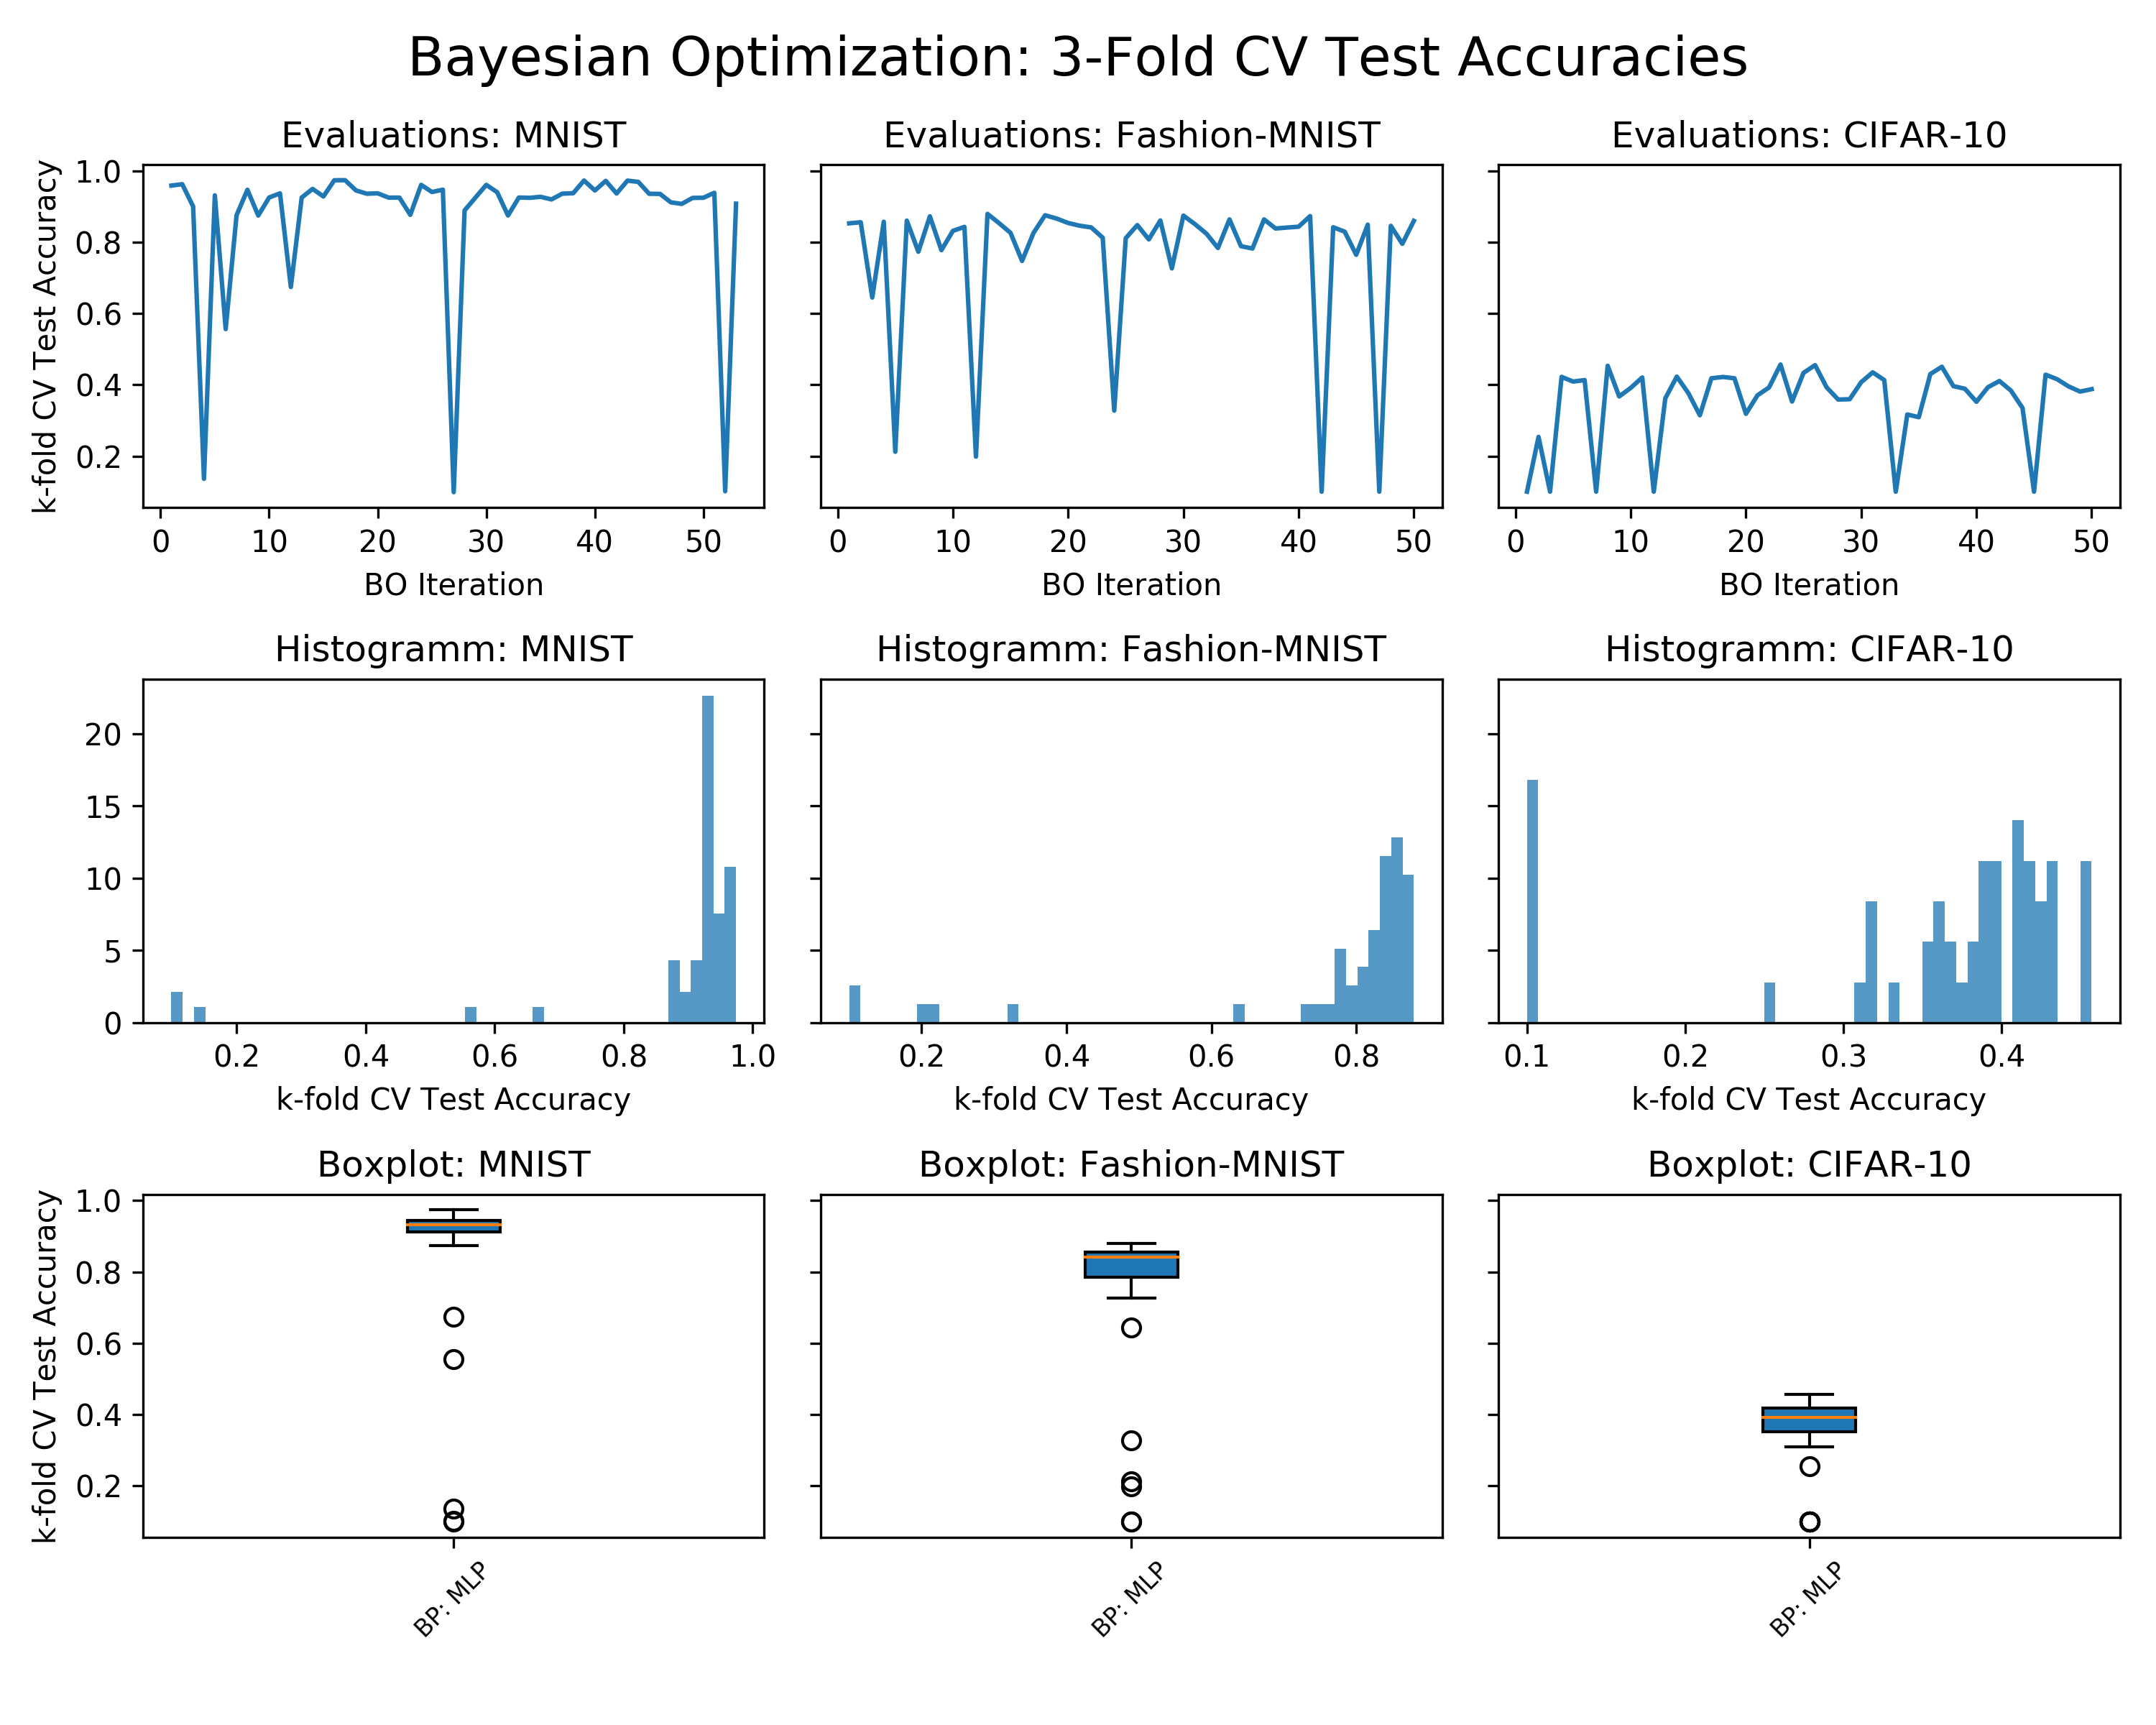
\includegraphics[width=\textwidth]{../figures/bayes_opt_comparison}
	\caption{Illustration of the learning performance. 50 runs of the BO scheme using a Matern kernel ($\nu=2.5$) and a UCB acquisition function. We display the time-series, histogram and boxplots for all models and datasets.}\label{fig:bo}
\end{figure}

In figure \ref{fig:bo} we display the results of a BO run with 50 evaluations for all three datasets (MNIST, Fashion-MNIST, CIFAR-10) as well as the three model types (backpropagation MLP and CNN as well as compartmental MLP)\footnote{As of the submission deadline we can only report 41, 30 and 23 BO iterations for the compartmental rule on the MNIST, Fashion-MNIST and CIFAR-10 dataset, respectively.}. The first row depicts the time-series of 3-fold cross-validated test accuracies throughout the optimization procedure. The second row, on the other hand, displays the discrete histogram of test accuracies. And finally, the last row demonstrates boxplots of the distributions. We can observe that both the traditional MLP and the CNN appear very robust across the different hyperparameters. The compartmental approach, on the other hand, does not appear very robust to changes from the reported hyperparameter constellation by \citet{guerguiev2017}. The distribution of 3-fold test accuracies obtained by the hyperparameter search exhibits large variance compared to the ones obtained from using backpropagation. 

%--------------------------------------------------------------------
\section{Outlook and Conclusion}

This report has empirically investigated the scalability and robustness of the compartmental alternative to backpropagation proposed by \citet{guerguiev2017}. We first reviewed the biological problems of implementing backpropagation in the brain. Then we discussed current approaches from the literature to circumvent such (e.g. feedback alignment \citep{lillicrap2016} and target propagation \citep{lee2015}). Afterwards, we turned towards a novel approach utilizing the electrical segregation of apical, somatic and basal compartments in pyramidal neurons. We reviewed the model and learning architecture which was divided into a forward and target phase. 
Finally, we reimplemented the model and run several robustness checks as well further analyses on the model. Given the hyperparameters provided in the paper, we are able to replicate and extend the results of \citet{guerguiev2017}. We find that weights are many magnitudes larger than for the backpropagation case. Furthermore, the algorithm performs as good if not even better on the MNIST task. 
For more complex datasets the learning rule still works but does not perform as good. Furthermore, the learning appears to converge fairly fast (relative to the Frobenius norm of the weights) and overfitting due to large weights might be a concern.
Finally, our results show that the learning rule is not robust to changes in the many hyperparameters. Backpropagation networks have far less hyperparameters to tune and appear extremely robust to such. The electrically segregated architecture, on the other hand, has many more hyperparameter configurations which lead to a learning rule that does not learn at all.

A recent extension introduced by \citet{sacramento2018} is to construct dendritic microcircuits. Here apical dendrites also act as integration zones, but in this case no separate phases are needed. Local errors encode the mismatch between pre-synaptic input from lateral interneurons and top-down feedback. The errors arise from a mismatch between lateral local interneuron inputs and somatic activity. Thereby apical dendrites have an explicit error representation which can be computed by simultaneous integration of top-down excitation and lateral inhibition. This gets rid of the implausible assumption of two distinct phases of integration.

Furthermore, Blake Richards recently highlighted the potential of "multiplexing".\footnote{See his keynote talk at ICLR 2018: \url{https://www.youtube.com/watch?v=C_2Q7uKtgNs}} Multiplexing \citep{naud_2018} describes the ability of a neuron to simultaneously track the content of different pathways (e.g. feedforward and feedback). More specifically, the burst rate might encode for top-down supervision and the event rate might represent the bottom-up propagation of sensory input. By letting a unit in the network be represented by an ensemble of neurons, one might overcome the discrete plateau potential events.

Finally, we bring up the following question: Why should the brain implement a suboptimal \textbf{and} non-robust learning rule on a neurophysiological level? A simple answer to this is the flexibility that such an alternative architecture comes with. 
Usually, the deep learning community has focused on coming up with better architectures to achieve super-human performance in a given task. While doing so, backpropagation is taken for granted. But it might be more time efficient to have a local error rule that is able to accommodate for the severe architectural network complexity observed in the brain.

We conclude by acknowledging the accomplishments of \citet{guerguiev2017}. They provide a \textbf{more} plausible learning rule based on a rate network that is made up of compartmental neurons. The dynamics operate in near-continuous time and perform reasonably well for a specific parameter constellation. Looking forward we would love to see more work extending such ideas to spiking networks as well as more plausible non-phasic learning. 

%--------------------------------------------------------------------
\setlength{\bibsep}{4pt plus 0.3ex}

\bibliographystyle{ecta}%plainnat - dinat - aer - econometrics
{\footnotesize \bibliography{main.bib}}

%--------------------------------------------------------------------
\section*{Supplementary Material}

\subsection*{Bayesian Optimization Hyperparameter Spaces}

\fcolorbox{black}[HTML]{E9F0E9}{\parbox{\textwidth}{%
\small{
\begin{center}
\begin{tabular}{ |p{3cm}||p{3cm}|p{6cm}| }
 \hline
 \multicolumn{3}{|c|}{\textbf{MLP Hyperparameter Search Space:}} \\
 \hline
Hyperparameter & Range & Description\\
 \hline
 Batchsize & Integer: $[50, 500]$ & Number of data points in mini-batch\\
 Learning Rate & Float: $[0.0001, 0.05]$ & SGD learning rate\\
 \# Hidden Layers & Integer: $[1, 6]$ & \\ 
 \# Hidden Layer Units & Integer: $[30, 500]$ & \\ 
 \hline
\end{tabular}	
\end{center}
}}}

\fcolorbox{black}[HTML]{E9F0E9}{\parbox{\textwidth}{%
\small{
\begin{center}
\begin{tabular}{ |p{3cm}||p{3cm}|p{6cm}| }
 \hline
 \multicolumn{3}{|c|}{\textbf{CNN Hyperparameter Search Space:}} \\
 \hline
Hyperparameter & Range & Description\\
 \hline
 Batchsize & Integer: $[50, 500]$ & Number of data points in mini-batch\\
 Learning Rate & Float: $[0.0001, 0.05]$ & SGD learning rate\\
 \# Hidden Layers & Integer: $[1, 6]$ & \\ 
 Channels & Integer: $[3, 64]$ & \\
 Kernels & Integer: $[2, 10]$ & \\
 Stride & Integer: $[1, 3]$ & \\
 Padding & Integer: $[1, 3]$ & \\
 \hline
\end{tabular}	
\end{center}
}}}


\fcolorbox{black}[HTML]{E9F0E9}{\parbox{\textwidth}{%
\small{
\begin{center}
\begin{tabular}{ |p{3cm}||p{3cm}|p{6cm}| }
 \hline
 \multicolumn{3}{|c|}{\textbf{Compartmental DNN Hyperparameter Search Space:}} \\
 \hline
Hyperparameter & Range & Description\\
 \hline
Sparse Feedback & Boolean & Dropout 80\% of the weights\\
Conductances & Boolean & Conductances between soma and dendrites\\
Broadcast & Boolean & Feedback output to all hidden layers\\
Spiking Feedback & Boolean & \\
Spiking Feedforward & Boolean & \\
Symmetric Weights  & Boolean & Enforce symmetry\\
Noisy Symmetric W. & Boolean & Add noise to symmetric weights\\
Update Feedback W. & Boolean & Sparse feedback weights\\
Apical conductances & Boolean & Attenuated conductances apical to soma\\
Weight Optimization & Boolean & Optimize initial weights\\
Feedback Bias & Boolean & Biases in feedback weights\\
$dt$  & Float: [0, 1]& Integration time step\\
Spike Memory & Integer: $[0, 10]$ & \\
Length Forward Train & Integer: $[2, 50]$ & \\
Length Target Phase & Integer: $[2, 50]$ & \\
Length Forward Test & Integer: $[50, 100]$ &\\
$\lambda_{max}$ & Float: $[0.2, 0.5]$ & Max spike rate per time step\\
$\tau_s$ & Float: $[1, 5]$ & Synaptic time constant \\
$\tau_L$ & Float: $[7, 13]$ & Leak time constant \\
$g_B$ & Float: $[0.3, 0.9]$ & Basal conductance \\
$g_A$ & Float: $[0.02, 0.1]$ & Apical conductance \\
$E_E$ & Float: $[5, 12]$ & Excitatory Reversal Potential \\
$E_I$ & Float: $[-12, -5]$ & Inhibitory Reversal Potential \\
Forward Learning R. & Float: $[0.01, 0.05]$ & SGD learning rate for forward weights\\
Backward Learning R. & Float: $[0, 0.05]$ & SGD learning rate for backward weights\\
 \# Hidden Layers & Integer: $[1, 6]$ & \\ 
 \# Hidden Layer Units & Integer: $[30, 500]$ & \\ 
 \hline
\end{tabular}	
\end{center}
}}}

\subsection*{Notes on Reproduction}

Please clone the repository \url{https://github.com/RobertTLange/Bio-Plausible-DeepLearning} and follow the instructions outlined below:
\hypertarget{repository-structure}{%
\subsection*{Repository Structure}\label{repository-structure}}

\begin{verbatim}
Bio-Plausible-DeepLearning
|-- workspace_dnn.ipynb: Train backpropagation MLP/CNN models and runs BO pipeline for them.
|-- workspace_comp_dnn.ipynb: Train individual compartmental MLP models.
|-- workspace_comp_visualize.ipynb: Produces the figures.
|-- run_bo.py: Script for Bayesian Optimization.
|-- figures: Folder containing saved figures.
|-- logs: Folder containing training and optimization logs
|-- models: Folder containing scripts defining DNN/CNN/CompDNN models
|-- report: Folder containing writeup and presentation slides
|-- utils: Helper functions (data preparation, logging, plotting, BO)
|-- Readme.md: Documentation
|-- requirements.txt: Dependencies
\end{verbatim}

\hypertarget{basic-how-to-use-this-code}{%
\subsection*{(Basic) How to use this
code}\label{basic-how-to-use-this-code}}

\begin{enumerate}
\def\labelenumi{\arabic{enumi}.}
\tightlist
\item
  Clone the repo.
\end{enumerate}

\begin{verbatim}
git clone https://github.com/RobertTLange/Bio-Plausible-DeepLearning
cd Bio-Plausible-DeepLearning
\end{verbatim}

\begin{enumerate}
\def\labelenumi{\arabic{enumi}.}
\setcounter{enumi}{1}
\tightlist
\item
  Create a virtual environment (optional but recommended).
\end{enumerate}

\begin{verbatim}
virtualenv -p python BioDL
\end{verbatim}

Activate the env (the following command works on Linux, other operating
systems might differ):

\begin{verbatim}
source BioDL/bin/activate
\end{verbatim}

\begin{enumerate}
\def\labelenumi{\arabic{enumi}.}
\setcounter{enumi}{2}
\tightlist
\item
  Install all dependencies:
\end{enumerate}

\begin{verbatim}
pip install -r requirements.txt
\end{verbatim}

\begin{enumerate}
\def\labelenumi{\arabic{enumi}.}
\setcounter{enumi}{3}
\tightlist
\item
  Run the main notebooks:
\end{enumerate}

\begin{verbatim}
jupyter notebook workspace_dnn.ipynb
jupyter notebook workspace_guergiev.ipynb
\end{verbatim}

\begin{enumerate}
\def\labelenumi{\arabic{enumi}.}
\setcounter{enumi}{4}
\tightlist
\item
  Run the bayesian optimization pipeline separately for compartmental
  DNN:
\end{enumerate}

\begin{verbatim}
python run_bo.py -t comp_dnn -d mnist
python run_bo.py -t comp_dnn -d fashion
python run_bo.py -t comp_dnn -d cifar10
\end{verbatim}

\begin{enumerate}
\def\labelenumi{\arabic{enumi}.}
\setcounter{enumi}{5}
\tightlist
\item
  Run the visualization notebook:
\end{enumerate}

\begin{verbatim}
jupyter notebook workspace_visualize.ipynb
\end{verbatim}

\hypertarget{advanced-jupyter-env-on-aws-ec2-instance-setup}{%
\subsection*{(Advanced) Jupyter Env on AWS EC2 Instance
Setup}\label{advanced-jupyter-env-on-aws-ec2-instance-setup}}

During the course of this project I trained many models. More
specifically, I run 50 iterations of the BO pipeline for all three
analyzed datasets as well as all three model types (Backprop MLP,
Backprop CNN, Segregated Comp MLP). Running the Bayesian Optimization
(BO) pipeline takes a while. Therefore, I run most of the analysis on a
\textbf{p2.xlarge} AWS EC2 instance which utilizes a Tesla K80 GPU. In
total training should take no more than 24 hours. Depending on the AMI
that you use and whether or not you use a demand/spot instance, this
should cost around 15\$. I recommend the AWS Deep Learning Base AMI.

\begin{enumerate}
\def\labelenumi{\arabic{enumi}.}
\tightlist
\item
  Clone repo, Create/Activate the environment and install dependencies
\end{enumerate}

\begin{verbatim}
git clone https://github.com/RobertTLange/Bio-Plausible-DeepLearning
cd Bio-Plausible-DeepLearning
conda create --name BioDL python=3.6 --no-default-packages
source activate BioDL
pip install -r requirements.txt --quiet
\end{verbatim}

\begin{enumerate}
\def\labelenumi{\arabic{enumi}.}
\setcounter{enumi}{1}
\tightlist
\item
  Add ipykernel to listed env kernels, Launch notebook silent and open
  port (start a screen session in between!)
\end{enumerate}

\begin{verbatim}
python -m ipykernel install --user --name BioDL --display-name "Python3 (BioDL)"
jupyter notebook --no-browser --port=8080
\end{verbatim}

\begin{enumerate}
\def\labelenumi{\arabic{enumi}.}
\setcounter{enumi}{2}
\tightlist
\item
  In new terminal window on local machine rewire port and listen
\end{enumerate}

\begin{verbatim}
ssh -i keyname.pem -N -f -L localhost:2411:localhost:8080 user@MACHINE_IP_ADDRESS
\end{verbatim}

\begin{enumerate}
\def\labelenumi{\arabic{enumi}.}
\setcounter{enumi}{3}
\tightlist
\item
  In Browser open localhost port and start working on the notebook of
  choice. If required copy paste the token/set a password. Afterwards
  run notebook of choice
\end{enumerate}

\begin{verbatim}
localhost:2411
\end{verbatim}

\begin{enumerate}
\def\labelenumi{\arabic{enumi}.}
\setcounter{enumi}{4}
\tightlist
\item
  After computations are done either git add, comnmit, push to remote
  repo or copy files back.
\end{enumerate}

\begin{verbatim}
scp -i keyname.pem -r user@MACHINE_IP_ADDRESS:Bio-Plausible-DeepLearning .
\end{verbatim}

\hypertarget{jupyter-env-cleanup}{%
\subsection*{Jupyter Env Cleanup}\label{jupyter-env-cleanup}}

\begin{verbatim}
conda env remove -n BioDL
jupyter kernelspec uninstall BioDL
\end{verbatim}


\end{document}